\subsection{Subsystem Decomposition}
\begin{figure}[H]
	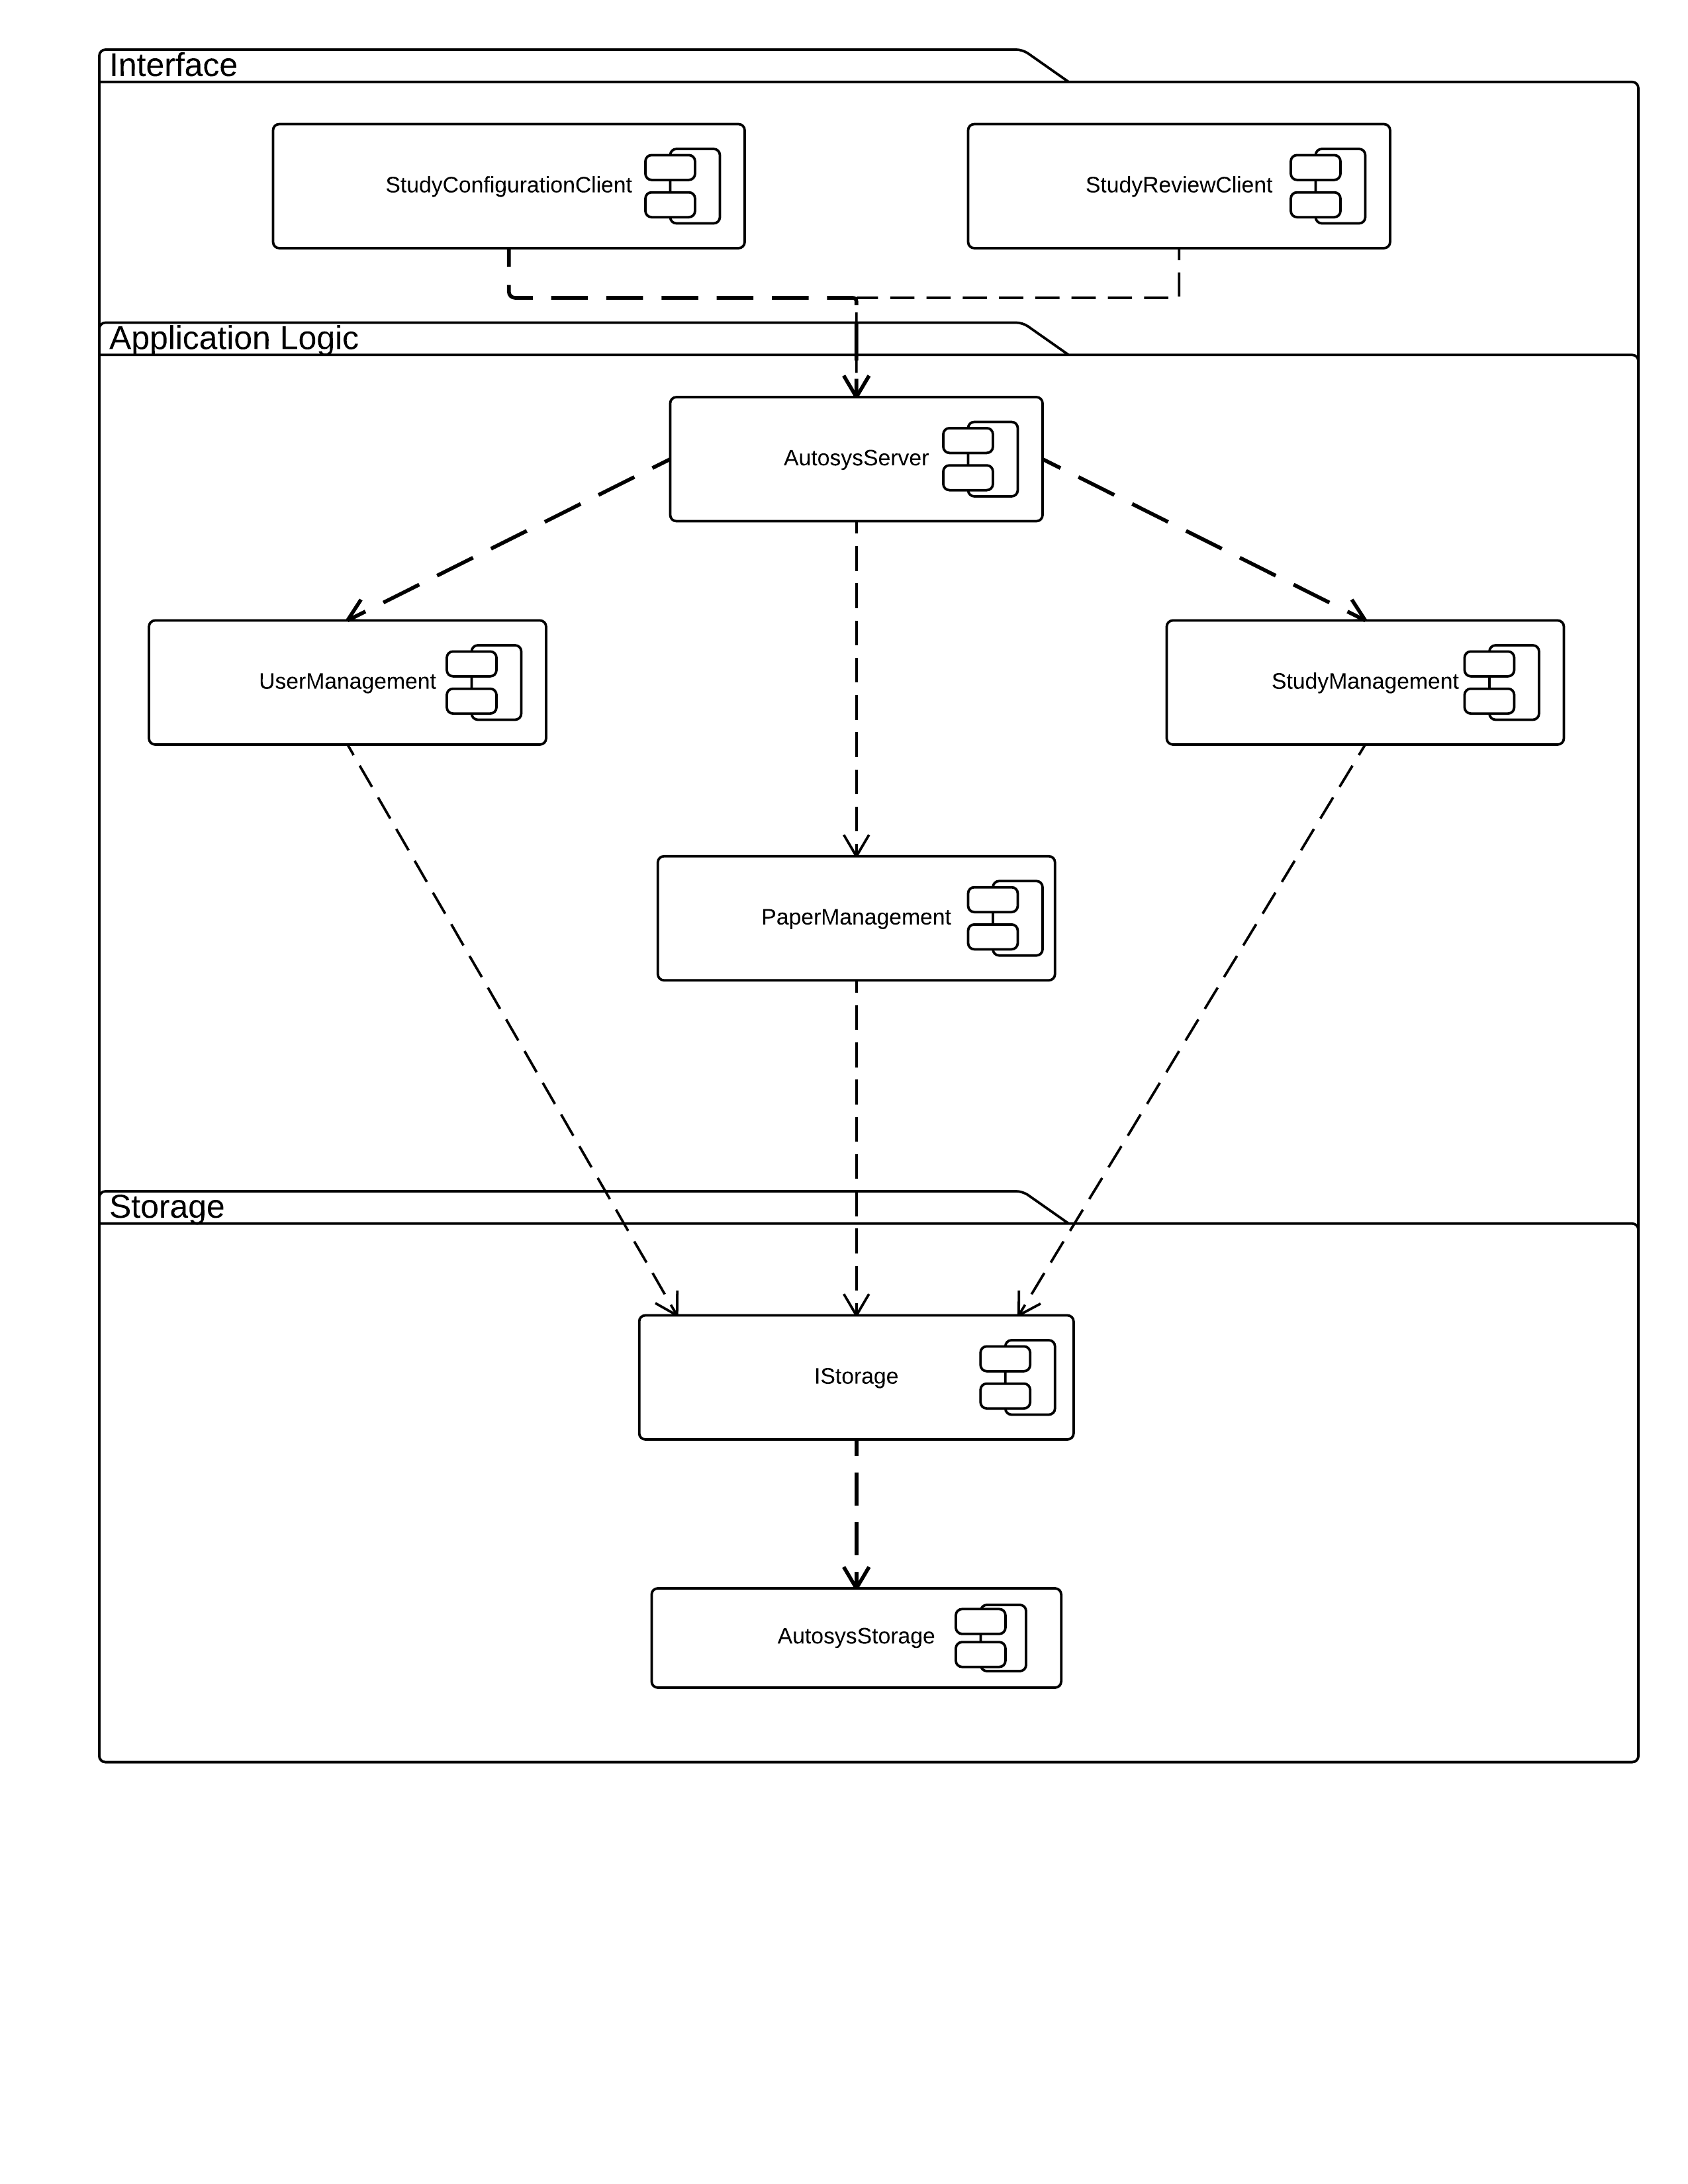
\includegraphics[width = \linewidth]{UMLComponentDiagramSubsystems}
	\caption{Autosys subsystem decomposition (UML Component Diagram, layers shown as UML packages)}
	\label{fig:Subsystem Decomposition, UML Component Diagram}
\end{figure}
The figure above shows a three-tier architectural style has been applied in the decomposition of the system. This architecture has been chosen instead of a two-tier client-server approach. Consequently, we avoid closely combining the application data and application logic on the server. The three-tier style results in a division into three independent tiers; Interface, Application Logic, and Storage. This makes it possible to update or change the individual tiers without affecting the whole application. In this way, the scaling and management of the system becomes more flexible as opposed to a client/server architectural style.
Finally, it is worth noting that still allows for high security and easier administration of the data through the centralized data access.\\
From the functional requirements of the Autosys RAD document, the following needed services are defined by grouping related operations that share a common purpose:\\
\begin{itemize}
	\item Study Configuration
	\item Task Handling
	\item Paper Screening
	\item Study Export
	\item User Validation
	\item User Management
	\item Research Protocol Generation
\end{itemize}
The \textbf{StudyConfigurationClient} provides the service related to configuring a study. It is a front end for users used to initiate all use cases related to setting up or configuring a \textbf{Study}.
The \textbf{ReviewService} provides an interface for different Review Clients to communicate with the \textbf{AutosysServer}, such that the system is not dependent on the review client - ultimately resulting in a more flexible design.
The \textbf{WebApi} will be providing the user validation services for allowing user access to all other Management components in the application logic (see Figure: \ref{fig:Subsystem Decomposition, UML Component Diagram}).
 From the \textbf{WebApi} a \textbf{ReviewServiceInterface} will be provided, which supports the use of an adapter pattern to communicate with different/changing client systems.
The \textbf{UserManagement} component is providing the user management service, since it holds the responsibility for handling all CRUD operations regarding teams and individual users. The \textbf{StudyManagement} component  provides the study configuration service by allowing users to set up and manage study information.
The \textbf{ExportMangement} provides the study export service allowing users to export Studies as plain data sets, e.g. csv files.
The \textbf{PaperManagement} provides the paper screening service by running filtering mechanisms on the research papers to get relevant papers according to the Study Criteria and Classifications.
The \textbf{ProtocolManagement} provides the services related to generating a Research Protocol and manages export of protocols to studies based on their configuration. 
The\textbf{ Storage} interface is used to decouple the storage abstraction from the application logic so that the two can vary independently (Bridge Pattern). 
The \textbf{AutosysStorage} represents the subsystem for storing the user data, study data, and research papers.
All packages in the UML Diagram \ref{fig:Subsystem Decomposition, UML Component Diagram} symbolize different projects in the programmed system, and all components symbolize directories except the WebApi component which have been made a separate project outside of ApplicationLogics. This was due to the possible complications with compilation of files which could arise when trying to combine both a web application project and a console application in one project.
